\documentclass[a4paper,11pt,english]{article}
\usepackage[T1]{fontenc}
\usepackage[utf8]{inputenc}
\usepackage{lmodern}
\usepackage{graphicx}
\usepackage{babel,blindtext}
\usepackage{float}
\usepackage{wrapfig}	
\title{PH21 Assignment 3}
\author{Helen Xue}

\begin{document}

\maketitle

\section{3.1}
The two images I picked were "sheep" and "pikachu"; these images were pulled from the internet with python's requests library.

\begin{figure}[H]
\minipage{0.32\textwidth}
	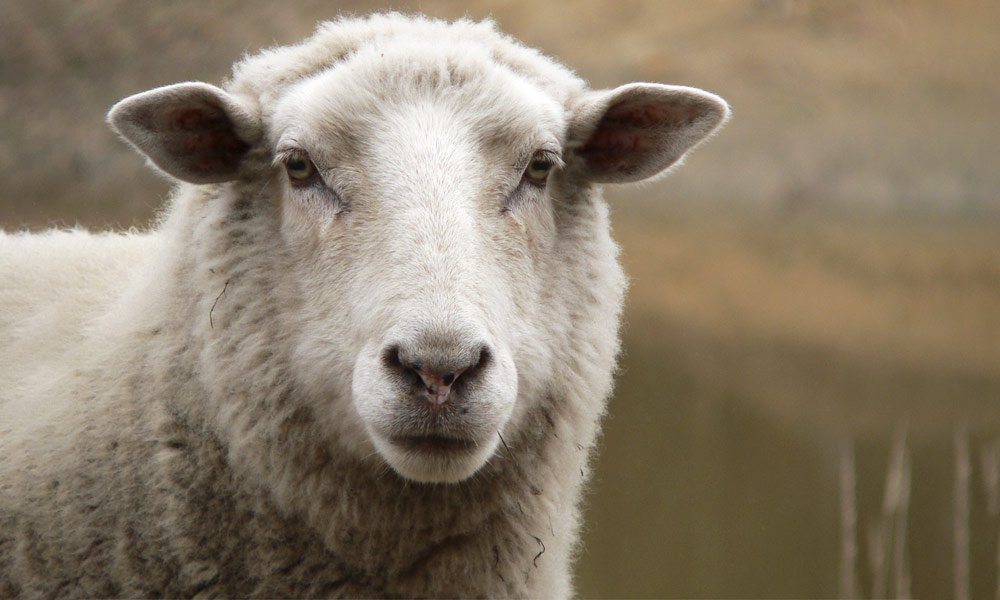
\includegraphics[width=\linewidth]{sheep/sheep}
	\caption{sheep}  
\endminipage \hfill
\minipage{0.32\textwidth}
	
\includegraphics[width=\linewidth]{pikachu/pikachu}
	\caption{pikachu} 
\endminipage \hfill
\end{figure}
\section{3.3-3.5}
I used the existing FIND$\_$EDGES image filters to make a demo; then I blurred the image and converted it to grayscale 
so that I could find the pixel brightness without distraction. Using these values, I 
used a built-in gaussian$\_$gradient function to measure the local derivative and find the edges.
\par Demo of possible effect:

\begin{figure}[H]
	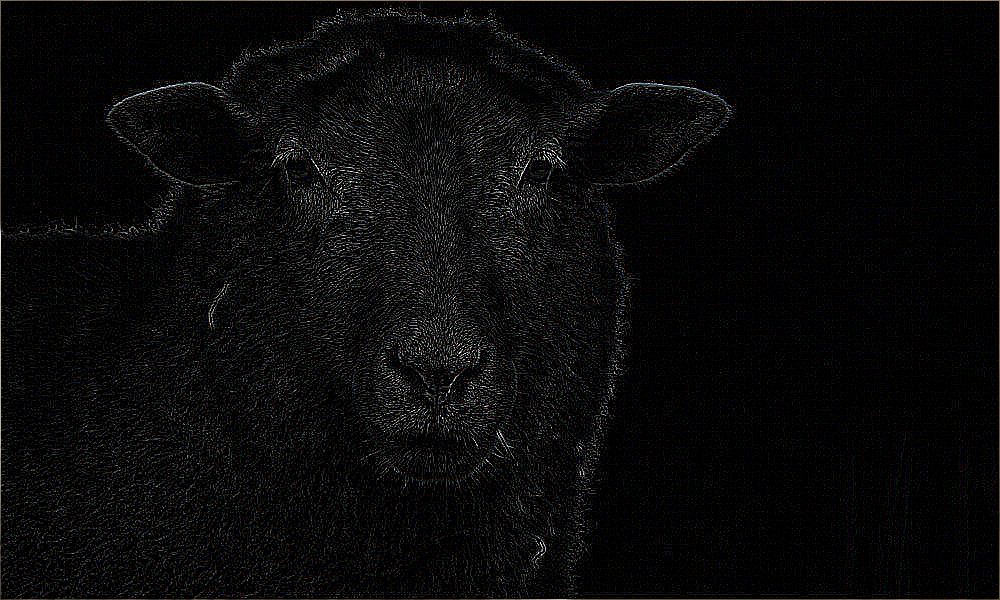
\includegraphics[width=\linewidth]{sheep/sheep_FIND_EDGES_demo}
	\caption{sheep demo}  
	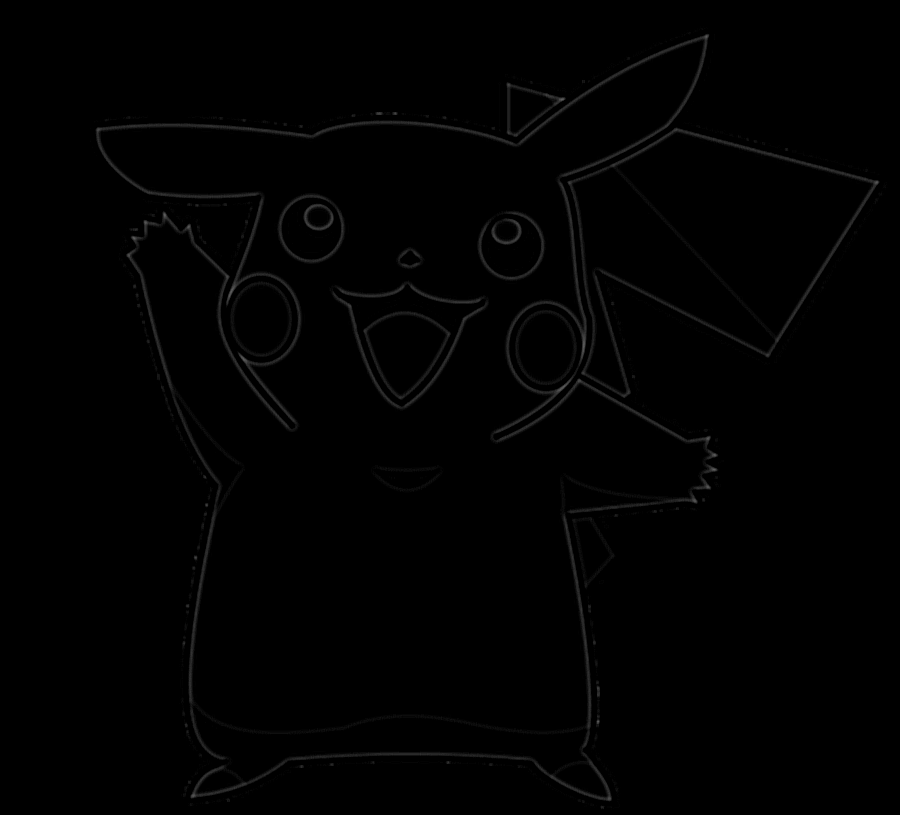
\includegraphics[width=\linewidth]{pikachu/pikachuFINDEDGESdemo}
	\caption{pikachu demo} 
\end{figure}

\par Results:
\begin{figure}[H]
	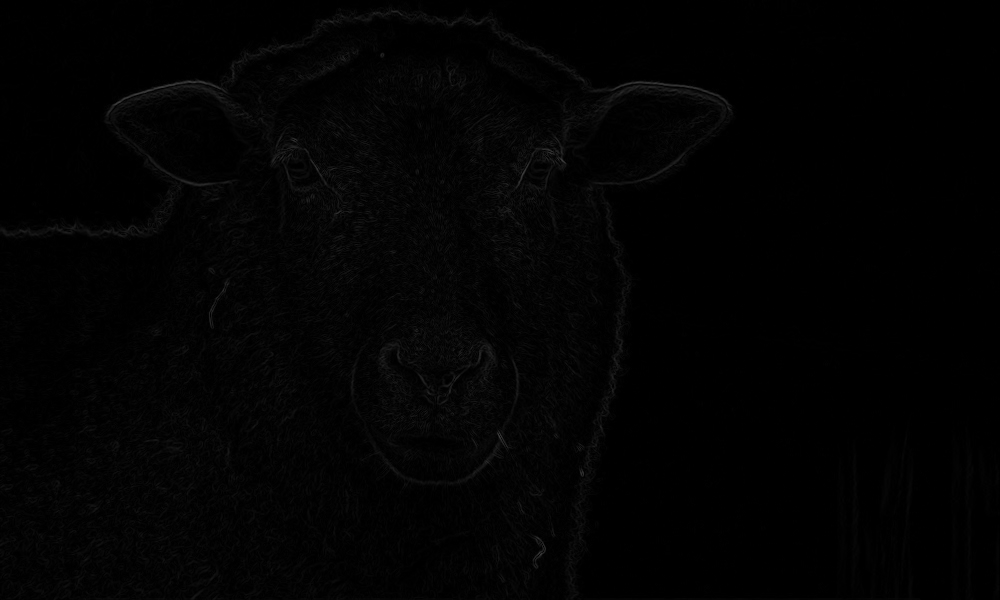
\includegraphics[width=\linewidth]{{sheep/sheep_width_0.6}.png}
	\caption{sheep results: no blur, $\sigma = 0.6$}  
	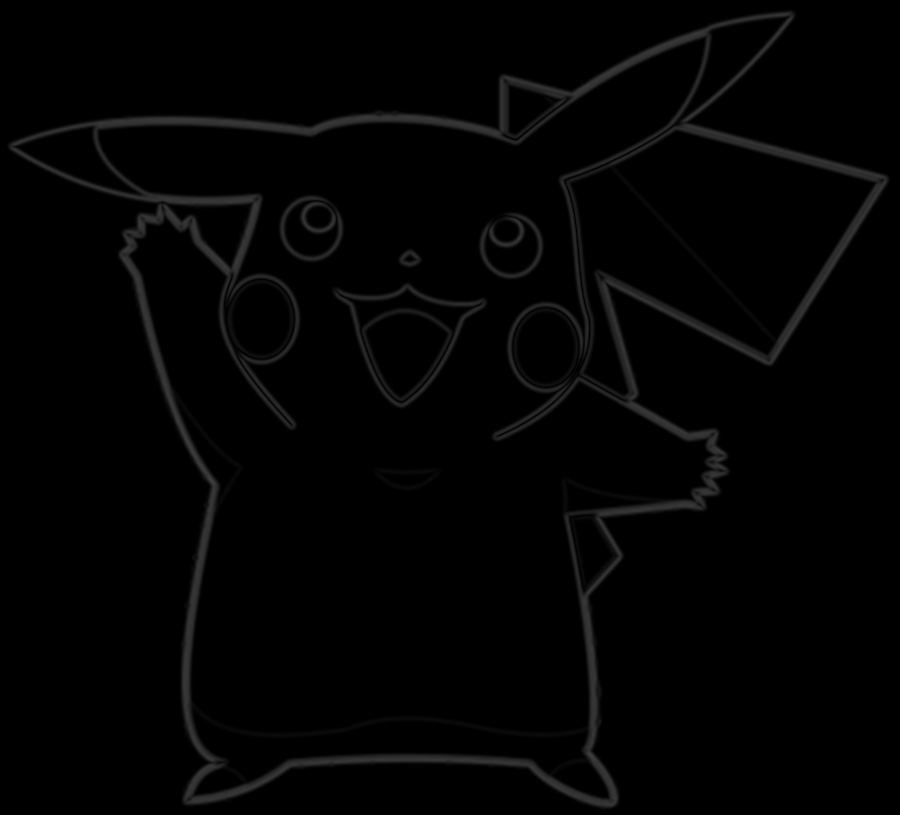
\includegraphics[width=\linewidth]{{pikachu/pikachu_width_0.6}.png}
	\caption{pikachu results: $\sigma = 0.6$} 
\end{figure}

The Pikachu results were pretty crisp; I think the fact that the image was against a clean background helped.
\par The sheep picture was no where near as good, partly because of the colored background. I chose to not blur the original picture before doing edge detection, since doing that lost much of the fur definition, which we can see very clearly in the demo and a little bit in my results.
\section{3.6}
\par Yes, we can probably use edge detection on captchas; edge detection will capture the shape of letters. If we have an extensive enough image bank of known letters, we could match shapes and figure out what the letters were. This is probably why most captchas have a lot of dots and stuff in the back; images with noise are harder to classify.

\section{3.7}
\par Edge detection seems really strong, although the image probably needs heavy pre-processing for best results in real life applications; in addition, it'd probably good to edge detect on several "types" of pixels, since differentiating using colors can double check the results from differentiating using brightness, or vice versa.
\par I think this assignment could be longer/clearer. The question text didn't really explain very much for the hard parts in the middle, and it wasn't immediately obvious what resources could be used and what couldn't ('skim[ming] the Wikipedia page' was allowed, but was reading the detailed implementations there ok?), and I was also unsure of what kind of built-in functions we could use (part 4 says 'convolve your image with a blurring filter'; I used PIL's built in Gaussian blur, was this ok? For the Gaussian gradient magnitude, I also used a built in function.) (This was resolved in section. Thank you!)
\par It was pretty cool to see the edges come out though. Fun assignment overall?
               
\end{document}
